% !TEX TS-program = pdflatex
% !TEX encoding = UTF-8 Unicode

% This is a simple template for a LaTeX document using the "article" class.
% See "book", "report", "letter" for other types of document.

\documentclass[11pt]{article} % use larger type; default would be 10pt

\usepackage[utf8]{inputenc} % set input encoding (not needed with XeLaTeX)

%%% Examples of Article customizations
% These packages are optional, depending whether you want the features they provide.
% See the LaTeX Companion or other references for full information.

%%% PAGE DIMENSIONS
\usepackage{geometry} % to change the page dimensions
\geometry{a4paper} % or letterpaper (US) or a5paper or....
\geometry{margin=1in} % for example, change the margins to 2 inches all round
% \geometry{landscape} % set up the page for landscape
%   read geometry.pdf for detailed page layout information

\usepackage{graphicx} % support the \includegraphics command and options

% \usepackage[parfill]{parskip} % Activate to begin paragraphs with an empty line rather than an indent
\usepackage{amssymb}
\usepackage{amsmath}
%%% PACKAGES
\usepackage{booktabs} % for much better looking tables
\usepackage{array} % for better arrays (eg matrices) in maths
\usepackage{paralist} % very flexible & customisable lists (eg. enumerate/itemize, etc.)
\usepackage{verbatim} % adds environment for commenting out blocks of text & for better verbatim
\usepackage{subfig} % make it possible to include more than one captioned figure/table in a single float
% These packages are all incorporated in the memoir class to one degree or another...

%%% HEADERS & FOOTERS
\usepackage{fancyhdr} % This should be set AFTER setting up the page geometry
\pagestyle{fancy} % options: empty , plain , fancy
\renewcommand{\headrulewidth}{0pt} % customise the layout...
\lhead{}\chead{}\rhead{}
\lfoot{}\cfoot{\thepage}\rfoot{}

%%% SECTION TITLE APPEARANCE
\usepackage{sectsty}
\allsectionsfont{\sffamily\mdseries\upshape} % (See the fntguide.pdf for font help)
% (This matches ConTeXt defaults)

%%% ToC (table of contents) APPEARANCE
\usepackage[nottoc,notlof,notlot]{tocbibind} % Put the bibliography in the ToC
\usepackage[titles,subfigure]{tocloft} % Alter the style of the Table of Contents
\usepackage{bbm}
\usepackage{endnotes}

\renewcommand{\cftsecfont}{\rmfamily\mdseries\upshape}
\renewcommand{\cftsecpagefont}{\rmfamily\mdseries\upshape} % No bold!
\DeclareMathOperator*{\argmax}{arg\,max}
\DeclareMathOperator*{\argmin}{arg\,min}

\usepackage{graphicx}
\graphicspath{ {./pings/} }

\newcount\colveccount
\newcommand*\colvec[1]{
        \global\colveccount#1
        \begin{pmatrix}
        \colvecnext
}
\def\colvecnext#1{
        #1
        \global\advance\colveccount-1
        \ifnum\colveccount>0
                \\
                \expandafter\colvecnext
        \else
                \end{pmatrix}
        \fi
}

\newcommand{\norm}[1]{\left\lVert#1\right\rVert}

\title{Computational Problem Set 6}
\author{Michael B. Nattinger, Sarah J. Bass, Xinxin Hu}

\begin{document}
\maketitle
\section{Solving for static choices}
The labor choice problem of the firm is the following: 
\begin{align*}
\pi(s;p) &= \max_{n\geq 0} psn^{\theta} - n - pc_f\\
\Rightarrow \theta psn^{\theta - 1} &= 1\\
\Rightarrow n &= (\theta p s)^{\frac{1}{1-\theta }} 
\end{align*}

The steady state equilibrium implies a static choice on the household side:
\begin{align*}
\max_{C,N} log(C) - AN \\
\text{s.t. } pC\leq N + \Pi \\
\Rightarrow \frac{1}{C} &= \lambda p, \lambda = A\\
\Rightarrow N &= \frac{1}{A} - \Pi.
\end{align*}

We computed the results. The table is as follows:

\begin{center}
\begin{tabular}{ll}
& Equilibrium \\ 
\hline 
Capital & 5.0451 \\ 
Wage & 1.1461 \\ 
Interest rate & 0.12778 \\ 
\hline 
\end{tabular}
\end{center}

Under the TV1 shocks, the price level is lower as the EV shocks increase value in expectations (this is a standard finding in IO, but in that context the presence of EV shocks improve welfare instead of profits. In order for the entry conditions to be satisfied the price level needs to drop to lower profitability back down. The mass of incumbents still ends up being a bit higher, however the mass of exits shoots up (as now there is 1) more mass overall and 2) firms from all states exit with positive probability). Labor levels are higher as there are more firms, and more firms in high-productivity states. Most of the increase in labor comes from the entrants, as the incumbents actually now demand slightly less labor (as more incumbent firms will be low productivity firms that received a high shock to not exiting). More entrants does imply more labor as the entrants have the same distribution (invariant distribution) of types, but have more mass entering. As a result, the fraction of labor in entrants is higher under the TV1 shocks. Note that the $\alpha = 2$ shock is somewhere in the middle of the standard version and $\alpha = 1$ versions, as anticipated.

We now document the exit rules:

\begin{center}
Figure 1: Exit probabilities, $c_F = 10$
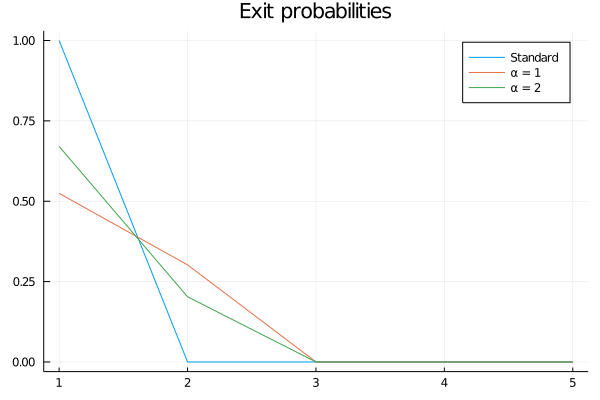
\includegraphics[scale=0.5]{exit_prob_1}

\bigskip

Figure 2: Exit probabilities, $c_F = 15$
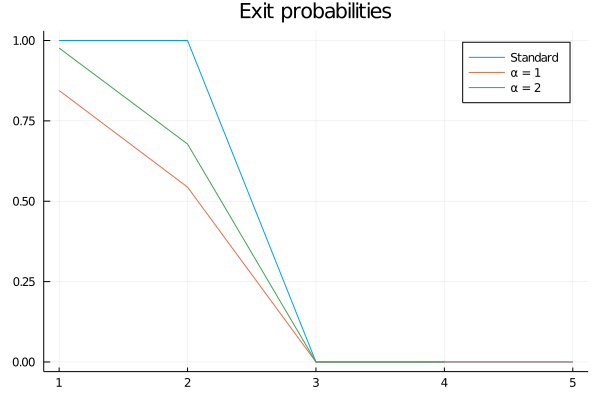
\includegraphics[scale=0.5]{exit_prob_2}
\end{center}

As we can see from our figures above, the standard version has state-dependent exit probabilities $\in \{0,1\}$ as their is no noise to their value of exiting and staying. Under the TV1, firms have some positive probability of exiting in any state, but essentially zero probability of exiting in states 3-5. State 2 has a sizable amount of exits, around 20-30 percent of firms exit between the two values of $\alpha$. When we change $c_F = 15$ then the cost of producing is substantially higher than before, and under the standard version all firms exit in states 1 and 2, not just 1. Under TV1, most firms in these stsates leave but a substantial chunk of firms in state 2 remain (roughly 30-40 percent across the two $\alpha$ values). Almost all firms in states 3, 4, and 5 stay in all versions. As before, the $\alpha = 2$ lies somewhere between $\alpha = 1$ and the standard version for all numbers and figures.
\end{document}
